\section{\IFRU{Инструкции}{Instructions}}
\label{sec:x86_instructions}

\IFRU{Инструкции, отмеченные как (M) обычно не генерируются компилятором: если вы видите её, вероятно,
это вручную написанный фрагмент кода, либо это т.н. compiler intrinsic}
{Instructions marked as (M) are not usually generated by compiler: if you see it, it is probably
hand-written piece of assembly code, or this is compiler intrinsic} (\ref{sec:compiler_intrinsic}).

% TODO ? обратные инструкции

\IFRU{Только наиболее используемые инструкции перечислены здесь}
{Only most frequently used instructions are listed here}.
\IFRU{Обращайтесь к}{Read} \cite{Intel} \OrENRU \cite{AMD} 
\IFRU{для полной документации}{for a full documentation}.

\subsection{\IFRU{Префиксы}{Prefixes}}

\begin{description}
\label{x86_lock}
\item[LOCK] \IFRU{используется чтобы предоставить эксклюзивный доступ к памяти в многопроцессорной среде}
{force CPU to make exclusive access to the RAM in multiprocessor environment}.
\IFRU{Для упрощения, можно сказать, что когда исполняется инструкция с этим префиксом, остальные процессоры
в системе останавливаются}{For the sake of simplification, it can be said that when instruction
with this prefix is executed, all other CPUs in multiprocessor system is stopped}.
\IFRU{Чаще все это используется для критических секций, семафоров, мьютексов}{Most often
it is used for critical sections, semaphores, mutexes}.
\IFRU{Обычно используется с}{Commonly used with} ADD, AND, BTR, BTS, CMPXCHG, OR, XADD, XOR.
\IFRU{Читайте больше о критических секциях}{Read more about critical sections} (\ref{critical_sections}).

\item[REP] \IFRU{используется с инструкциями}{used with} MOVSx \AndENRU STOSx\IFRU{ instructions}{}:
\IFRU{инструкция будет исполняться в цикле, счетчик расположен в регистре CX/ECX/RCX}
{execute the instruction in loop, counter is located in the CX/ECX/RCX register}.
\IFRU{Для более детального описания, читайте больше об инструкциях}
{For detailed description, read more about} MOVSx (\ref{REP_MOVSx}) 
\AndENRU STOSx (\ref{REP_STOSx})\EN{ instructions}.

\IFRU{Работа инструкций с префиксом REP зависит от флага DF, он задает направление}
{Instructions prefixed by REP are sensitive to DF flag, which is used to set direction}.

\item[REPE/REPNE] (\ac{AKA} REPZ/REPNZ) \IFRU{используется с инструкциями}{used with} CMPSx \AndENRU
SCASx\RU{ instructions}:
\IFRU{инструкция будет исполняться в цикле, счетчик расположен в регистре \TT{CX}/\TT{ECX}/\TT{RCX}}
{execute the last instruction in loop, count is set in the \TT{CX}/\TT{ECX}/\TT{RCX} register}. 
\IFRU{Выполнение будет прервано если ZF будет 0 (REPE) либо если ZF будет 1 (REPNE)}
{It will terminate prematurely if ZF is 0 (REPE) or if ZF is 1 (REPNE)}.

\IFRU{Для более детального описания, читайте больше об инструкциях}
{For detailed description, read more about} CMPSx (\ref{REPE_CMPSx}) 
\AndENRU SCASx (\ref{REPNE_SCASx})\EN{ instructions}.

\IFRU{Работа инструкций с префиксами REPE/REPNE зависит от флага DF, он задает направление}
{Instructions prefixed by REPE/REPNE are sensitive to DF flag, which is used to set direction}.

\end{description}

\subsection{\IFRU{Наиболее часто используемые инструкции}{Most frequently used instructions}}

\IFRU{Их можно заучить в первую очередь}{These can be memorized in the first place}.

\begin{description}
% in order to keep them easily sorted...
\index{x86!\Instructions!ADC}
  \item[ADC] (\IT{add with carry}) \IFRU{сложить два значения, \glslink{increment}{инкремент} 
  если выставлен флаг CF.
  часто используется для складывания больших значений, например, складывания двух 64-битных
  значений в 32-битной среде используя две инструкции ADD и ADC, например:}
  {add values, \gls{increment} result if CF flag is set.
  often used for addition of large values, for example, 
  to add two 64-bit values in 32-bit environment using two ADD and ADC instructions, for example:}

\lstinputlisting{appendix/x86/instructions/ADC_example_\IFRU{ru}{en}.lst}


\index{x86!\Instructions!ADD}
  \item[ADD] \IFRU{сложить два значения}{add two values}

\myindex{x86!\Instructions!AND}
  \item[AND] \RU{логическое \q{И}}\EN{logical \q{and}}

\index{x86!\Instructions!CALL}
  \item[CALL] \IFRU{вызвать другую ф-цию}{call another function}: \TT{PUSH address\_after\_CALL\_instruction; JMP label}

\index{x86!\Instructions!CMP}
  \item[CMP] \IFRU{сравнение значений и установка флагов, то же что и \TT{SUB}, но только без записи результата}
  {compare values and set flags, the same as \TT{SUB} but no results writing}

\index{x86!\Instructions!DEC}
\index{x86!\Flags!CF}
  \item[DEC] \gls{decrement}. \RU{Флаг CF не модифицируется}\EN{The CF flag is not modified}.

\index{x86!\Instructions!IMUL} 
  \item[IMUL] \IFRU{умножение с учетом знаковых значений}{signed multiply}

\index{x86!\Instructions!INC} 
  \item[INC] \gls{increment}. \RU{Флаг CF не модифицируется}\EN{CF flag is not touched}.

\myindex{x86!\Instructions!JCXZ}
\myindex{x86!\Instructions!JECXZ}
\myindex{x86!\Instructions!JRCXZ}
  \item[JCXZ, JECXZ, JRCXZ] (M) \RU{переход если CX/ECX/RCX=0}\EN{jump if CX/ECX/RCX=0}

\index{x86!\Instructions!JMP}
\item[JMP] \RU{перейти на другой адрес}\EN{jump to another address}.
\RU{Опкод имеет т.н.}\EN{Opcode has} \gls{jump offset}.

\item[Jcc] (\RU{где}\EN{where} cc\EMDASH{}condition code)

\myindex{x86!\Instructions!JAE}
\myindex{x86!\Instructions!JA}
\myindex{x86!\Instructions!JBE}
\myindex{x86!\Instructions!JB}
\myindex{x86!\Instructions!JC}
\myindex{x86!\Instructions!JE}
\myindex{x86!\Instructions!JGE}
\myindex{x86!\Instructions!JG}
\myindex{x86!\Instructions!JLE}
\myindex{x86!\Instructions!JL}
\myindex{x86!\Instructions!JNAE}
\myindex{x86!\Instructions!JNA}
\myindex{x86!\Instructions!JNBE}
\myindex{x86!\Instructions!JNB}
\myindex{x86!\Instructions!JNC}
\myindex{x86!\Instructions!JNE}
\myindex{x86!\Instructions!JNGE}
\myindex{x86!\Instructions!JNG}
\myindex{x86!\Instructions!JNLE}
\myindex{x86!\Instructions!JNL}
\myindex{x86!\Instructions!JNO}
\myindex{x86!\Instructions!JNS}
\myindex{x86!\Instructions!JNZ}
\myindex{x86!\Instructions!JO}
\myindex{x86!\Instructions!JPO}
\myindex{x86!\Instructions!JP}
\myindex{x86!\Instructions!JS}
\myindex{x86!\Instructions!JZ}

\RU{Немало этих инструкций имеют синонимы (отмечены с AKA), это сделано для удобства}
\EN{A lot of these instructions have synonyms (denoted with AKA), this was done for convenience}.
\RU{Синонимичные инструкции транслируются в один и тот же опкод}
\EN{Synonymous instructions are translated into the same opcode}.
\RU{Опкод имеет т.н.}\EN{The opcode has a} \gls{jump offset}.

\label{Jcc}
\begin{description}
\item[JAE] \ac{AKA} JNC: \RU{переход если больше или равно (беззнаковый)}\EN{jump if above or equal (unsigned)}: CF=0
\EN{\item[JA] \ac{AKA} JNBE: jump if greater (unsigned): CF=0 and ZF=0}
\RU{\item[JA] \ac{AKA} JNBE: переход если больше (беззнаковый): CF=0 и ZF=0}
\EN{\item[JBE] jump if lesser or equal (unsigned): CF=1 or ZF=1}
\RU{\item[JBE] переход если меньше или равно (беззнаковый): CF=1 или ZF=1}
\item[JB] \ac{AKA} JC: \RU{переход если меньше (беззнаковый)}\EN{jump if below (unsigned)}: CF=1
\item[JC] \ac{AKA} JB: \RU{переход если CF=1}\EN{jump if CF=1}
\item[JE] \ac{AKA} JZ: \RU{переход если равно или ноль}\EN{jump if equal or zero}: ZF=1
\item[JGE] \RU{переход если больше или равно (знаковый)}\EN{jump if greater or equal (signed)}: SF=OF
\EN{\item[JG] jump if greater (signed): ZF=0 and SF=OF}
\RU{\item[JG] переход если больше (знаковый): ZF=0 и SF=OF}
\EN{\item[JLE] jump if lesser or equal (signed): ZF=1 or SF$\neq$OF}
\RU{\item[JLE] переход если меньше или равно (знаковый): ZF=1 или SF$\neq$OF}
\item[JL] \RU{переход если меньше (знаковый)}\EN{jump if lesser (signed)}: SF$\neq$OF
\item[JNAE] \ac{AKA} JC: \RU{переход если не больше или равно (беззнаковый)}\EN{jump if not above or equal (unsigned)} CF=1
\item[JNA] \RU{переход если не больше (беззнаковый)}\EN{jump if not above (unsigned)} CF=1 \AndENRU ZF=1
\item[JNBE] \RU{переход если не меньше или равно (беззнаковый)}\EN{jump if not below or equal (unsigned)}: CF=0 \AndENRU ZF=0
\item[JNB] \ac{AKA} JNC: \RU{переход если не меньше (беззнаковый)}\EN{jump if not below (unsigned)}: CF=0
\item[JNC] \ac{AKA} JAE: \RU{переход если CF=0, синонимично}\EN{jump CF=0 synonymous to} JNB.
\item[JNE] \ac{AKA} JNZ: \RU{переход если не равно или не ноль}\EN{jump if not equal or not zero}: ZF=0
\item[JNGE] \RU{переход если не больше или равно (знаковый)}\EN{jump if not greater or equal (signed)}: SF$\neq$OF
\EN{\item[JNG] jump if not greater (signed): ZF=1 or SF$\neq$OF}
\RU{\item[JNG] переход если не больше (знаковый): ZF=1 или SF$\neq$OF}
\item[JNLE] \RU{переход если не меньше (знаковый)}\EN{jump if not lesser (signed)}: ZF=0 \AndENRU SF=OF
\item[JNL] \RU{переход если не меньше (знаковый)}\EN{jump if not lesser (signed)}: SF=OF
\item[JNO] \RU{переход если не переполнение}\EN{jump if not overflow}: OF=0
\item[JNS] \RU{переход если флаг SF сброшен}\EN{jump if SF flag is cleared}
\item[JNZ] \ac{AKA} JNE: \RU{переход если не равно или не ноль}\EN{jump if not equal or not zero}: ZF=0
\item[JO] \RU{переход если переполнение}\EN{jump if overflow}: OF=1
\item[JPO] \RU{переход если сброшен флаг PF}\EN{jump if PF flag is cleared} (Jump Parity Odd)
\item[JP] \ac{AKA} \ac{JPE}: \RU{переход если выставлен флаг PF}\EN{jump if PF flag is set}
\item[JS] \RU{переход если выставлен флаг SF}\EN{jump if SF flag is set}
\item[JZ] \ac{AKA} JE: \RU{переход если равно или ноль}\EN{jump if equal or zero}: ZF=1
\end{description}


\index{x86!\Instructions!LAHF}
  \item[LAHF] \IFRU{скопировать некоторые биты флагов в AH}{copy some flag bits to AH}

\myindex{x86!\Instructions!LEAVE}
\label{x86_ins:LEAVE}
\item[LEAVE] \RU{аналог команд \TT{MOV ESP, EBP} и \TT{POP EBP}\EMDASH{}
то есть возврат \glslink{stack pointer}{указателя стека} и регистра \EBP в первоначальное состояние.} 
\EN{equivalent of the \TT{MOV ESP, EBP} and \TT{POP EBP} instruction 
pair\EMDASH{}in other words, this instruction sets the \gls{stack pointer} (\ESP) back and restores 
the \EBP register to its initial state.}


\index{x86!\Instructions!LEA}
  \item[LEA] \IFRU{сформировать адрес}{form address} \IFRU{см.также}{see also}: \ref{sec:LEA}

% to be proofreaded
\index{\CStandardLibrary!memcpy()}
\index{x86!\Instructions!MOVSB}
\index{x86!\Instructions!MOVSW}
\index{x86!\Instructions!MOVSD}
\index{x86!\Instructions!MOVSQ}
\item[MOVSB/MOVSW/MOVSD/MOVSQ] 
\IFRU{скопировать}{copy} \IFRU{байт}{byte}/
16-\IFRU{битное слово}{bit word}/
32-\IFRU{битное слово}{bit word}/
64-\IFRU{битное слово}{bit word} \IFRU{на который указывает}{address of which is in the} SI/ESI/RSI 
\IFRU{куда указывает}{into the place address of which is in the} DI/EDI/RDI.

\label{REP_MOVSx}
\IFRU{Вместе с префиксом REP, инструкция будет исполняться в цикле, счетчик будет
находится в регистре CX/ECX/RCX}
{Together with REP prefix, it will repeated in loop, count is stored in the CX/ECX/RCX register}:
\IFRU{это работает как}{it works like} memcpy() \IFRU{в Си}{in C}.
\IFRU{Если размер блока известен компилятору на стадии компиляции,
memcpy() часто компилируется в короткий фрагмент кода использующий
REP MOVSx, иногда даже несколько инструкций}
{If block size is known to compiler on compile stage, 
memcpy() is often inlined into short code fragment
using REP MOVSx, sometimes even as several instructions}.

\IFRU{Эквивалент }{}memcpy(EDI, ESI, 15)\IFRU{}{ equivalent is}:

\lstinputlisting{appendix/x86/instructions/MOVSB_ex1_\IFRU{ru}{en}.asm}

(\IFRU{Вероятно, так быстрее чем копировать 15 байт используя просто одну}
{Supposedly, it will work faster then copying 15 bytes using just one} REP MOVSB).


\index{x86!\Instructions!MOVSX}
  \item[MOVSX] \IFRU{загрузить с расширением знака}{load with sign extension} \IFRU{см.также}{see also}: (\ref{MOVSX})

\myindex{x86!\Instructions!MOVZX}
  \item[MOVZX] \RU{загрузить и очистить все остальные биты}\EN{load and clear all other bits} \RU{см. также}\EN{see also}: (\myref{movzx})

\myindex{x86!\Instructions!MOV}
\item[MOV] \RU{загрузить значение}\EN{load value}. \RU{эта инструкция была названа неудачно 
(данные не перемещаются, а копируются), 
что является результатом путаницы: 
в других архитектурах эта же инструкция называется \q{LOAD} и/или \q{STORE} или что-то в этом роде.}
\EN{this instruction name is misnomer, resulting in some confusion (data is not moved but copied), 
in other architectures the same instructions is usually named \q{LOAD} and/or \q{STORE} or something like that.}

\RU{Важно: если в 32-битном режиме при помощи MOV записывать младшую 16-байтную часть регистра,
то старшие 16 бит останутся такими же.}
\EN{One important thing: if you set the low 16-bit part of a 32-bit register in 32-bit mode, the high 16 bits
remains as they were.}
\RU{Но если в 64-битном режиме модифицировать 32-битную часть регистра, то старшие 32 бита обнуляются.}
\EN{But if you modify the low 32-bit part of the register in 64-bit mode, 
the high 32 bits of the register will be cleared.}

\RU{Вероятно, это сделано для упрощения портирования кода под x86-64.}
\EN{Supposedly, it was done to simplify porting code to x86-64.}

\ifdefined\BRAZILIAN
% TODO to be resynced:
Como curiosidade, vale ressaltar que \MOV é um nome equivocado para a instrução em ambos conjuntos de intruções do x86 e ARM, pois a informação não é de fato movida e sim copiada para o registrador ou variável de destino.
\fi % BRAZILIAN


\index{x86!\Instructions!MUL}
  \item[MUL] \RU{умножение с учетом беззнаковых значений}\EN{unsigned multiply}

\myindex{x86!\Instructions!NEG}
  \item[NEG] \RU{смена знака}\EN{negation}: $op=-op$
\EN{Same as \TT{NOT op / ADD op, 1}.}
\RU{То же что и \TT{NOT op / ADD op, 1}.}


\index{x86!\Instructions!NOP}
  \item[NOP] \ac{NOP}. \IFRU{Её опкод 0x90, что на самом деле это холостая инструкция}
  {Opcode is 0x90, so it is in fact mean} 
  \TT{XCHG EAX,EAX}\IFRU{}{ idle instruction}.
  \IFRU{Это значит что в x86 (как и во многих \ac{RISC}) нет отдельной \ac{NOP}-инструкции}
  {This means, x86 do not have dedicated \ac{NOP} instruction (as in many \ac{RISC})}.
  \IFRU{Еще примеры подобных операций}{More examples of such operations}:
  (\ref{sec:npad})

\index{x86!\Instructions!NOT}
  \item[NOT] op1: $op1=\neg{}op1$. \RU{логическое \q{НЕ}}\EN{logical inversion}
  \RU{Особенность --- инструкция не меняет флаги.}
  \EN{Feature --- the instruction doesn't change flags.}

\myindex{x86!\Instructions!OR}
  \item[OR] \RU{логическое \q{ИЛИ}}\EN{logical \q{or}}

\myindex{x86!\Instructions!POP}
\EN{\item[POP] get a value from the stack: \TT{value=SS:[ESP]; ESP=ESP+4 (or 8)}}%
\RU{\item[POP] взять значение из стека: \TT{value=SS:[ESP]; ESP=ESP+4 (или 8)}}


\index{x86!\Instructions!PUSH}
\item[PUSH] \RU{записать значение в стек}\EN{push value to stack}: 
\TT{ESP=ESP-4 (\OrENRU 8); SS:[ESP]=value}

\index{x86!\Instructions!RET}
\index{MS-DOS}
\item[RET] \RU{возврат из процедуры}\EN{return from subroutine}: \TT{POP tmp; JMP tmp}.

\RU{В реальности}\EN{In fact}, RET 
\RU{это макрос ассемблера, в среде Windows и *NIX транслирующийся в}
\EN{is a assembly language macro, in Windows and *NIX environment is translating into}
RETN (``return near'') 
\RU{ибо, во времена MS-DOS, где память адресовалась немного иначе}
\EN{or, in MS-DOS times, where memory was addressed differently}
(\ref{8086_memory_model}), \RU{в}\EN{into} RETF (``return far'').

\TT{RET} \RU{может иметь операнд}\EN{may have operand}.
\RU{Тогда его работа будет такой}\EN{Its algorithm then will be}: \TT{POP tmp; ADD ESP op1; JMP tmp}.
\TT{RET} \RU{с операндом обычно завершает ф-ции с соглашением о вызовах \IT{stdcall}, см. также}
\EN{with operand usually end functions with \IT{stdcall} calling convention, see also}: \ref{sec:stdcall}.


\myindex{x86!\Instructions!SAHF}
\myindex{x86!\Registers!AH}

  \item[SAHF] \RU{скопировать биты из AH в флаги CPU}\EN{copy bits from AH to CPU flags}:

\begin{center}
\begin{bytefield}[endianness=big,bitwidth=0.03\linewidth]{8}
\bitheader{7,6,4,2,0} \\
\bitbox{1}{SF} & 
\bitbox{1}{ZF} & 
\bitbox{1}{} & 
\bitbox{1}{AF} & 
\bitbox{1}{} & 
\bitbox{1}{PF} & 
\bitbox{1}{} & 
\bitbox{1}{CF}
\end{bytefield}
\end{center}


\RU{Эта инструкция часто используется в коде работающем с \ac{FPU}.}
\EN{This instruction is often used in \ac{FPU}-related code.}


\index{x86!\Instructions!SBB}
  \item[SBB] (\IT{subtraction with borrow}) 
  \IFRU{вычесть одно значение из другого, \glslink{decrement}{декремент} результата если флаг CF выставлен.
  часто используется для вычитания больших значений, например, для вычитания двух 64-битных
  значений в 32-битной среде используя инструкции SUB и SBB, например:}
  {subtract values, \gls{decrement} result if CF flag is set.
  often used for subtraction of large values, for example,
  to subtract two 64-bit values in 32-bit environment using two SUB and SBB instructions, for example:}

\lstinputlisting{appendix/x86/instructions/SBB_example_\LANG.lst}

\IFRU{Еще один пример}{One more example}: \ref{sec:64bit_in_32_env}.

\index{\CStandardLibrary!strlen()}
\index{\CStandardLibrary!memchr()}
\index{x86!\Instructions!SCASB}
\index{x86!\Instructions!SCASW}
\index{x86!\Instructions!SCASD}
\index{x86!\Instructions!SCASQ}
\item[SCASB/SCASW/SCASD/SCASQ] (M) \RU{сравнить}\EN{compare} \RU{байт}\EN{byte}/
16-\RU{битное слово}\EN{bit word}/
32-\RU{битное слово}\EN{bit word}/
64-\RU{битное слово}\EN{bit word} \RU{записанный в}\EN{stored in the}
AX/EAX/RAX \RU{со значением, адрес которого находится
в}\EN{with a variable address of which is in the} DI/EDI/RDI.
\RU{Выставить флаги так же, как это делает \CMP}\EN{Set flags as \CMP does}.

\label{REPNE_SCASx}
\RU{Эта инструкция часто используется с префиксом REPNE: продолжать сканировать буфер до тех
пор, пока не встретится специальное значение, записанное в AX/EAX/RAX}
\EN{This instruction is often used with REPNE prefix: continue to scan a buffer until a special value
stored in AX/EAX/RAX is found}.
\RU{Отсюда ``NE'' в REPNE: продолжать сканирование если сравниваемые значения не равны и остановиться
если равны}
\EN{Hence ``NE'' in REPNE: continue to scan if compared values are not equal and stop when equal}.

\RU{Она часто используется как стандартная ф-ция Си strlen(), для определения длины \ac{ASCIIZ}-строки}
\EN{It is often used as strlen() C standard function, to determine \ac{ASCIIZ} string length}:

\RU{Пример}\EN{Example}:

\lstinputlisting{appendix/x86/instructions/SCASB_ex1_\LANG.asm}

\RU{Если использовать другое значение AX/EAX/RAX, ф-ция будет работать как стандартная ф-ция Си memchr(),
т.е., для поиска определенного байта}
\EN{If to use different AX/EAX/RAX value, the function will act as memchr() standard C function, i.e.,
it will find specific byte}.


\index{x86!\Instructions!SHL}
\index{x86!\Instructions!SHR}
  \item[SHL] \IFRU{сдвинуть значение влево}{shift value left}
  \item[SHR] \IFRU{сдвинуть значение вправо}{shift value right}:

\begin{center}
	\begin{tikzpicture}[scale=0.7, every node/.style={scale=0.7}]
	\edef\bitsize{1cm}
	\tikzstyle{byte}=[draw,minimum size=\bitsize]	
	\tikzstyle{every path}=[thick]

	\node [draw,rectangle,minimum size=\bitsize] (a1) {7};
	\node [draw,rectangle,minimum size=\bitsize] (a2) [right of=a1] {6};
	\node [draw,rectangle,minimum size=\bitsize] (a3) [right of=a2] {5};
	\node [draw,rectangle,minimum size=\bitsize] (a4) [right of=a3] {4};
	\node [draw,rectangle,minimum size=\bitsize] (a5) [right of=a4] {3};
	\node [draw,rectangle,minimum size=\bitsize] (a6) [right of=a5] {2};
	\node [draw,rectangle,minimum size=\bitsize] (a7) [right of=a6] {1};
	\node [draw,rectangle,minimum size=\bitsize] (a8) [right of=a7] {0};

	\node (empty) [below of=a1] {};

	\node [draw,rectangle,minimum size=\bitsize] (b1) [below of=empty] {7};
	\node [draw,rectangle,minimum size=\bitsize] (b2) [right of=b1] {6};
	\node [draw,rectangle,minimum size=\bitsize] (b3) [right of=b2] {5};
	\node [draw,rectangle,minimum size=\bitsize] (b4) [right of=b3] {4};
	\node [draw,rectangle,minimum size=\bitsize] (b5) [right of=b4] {3};
	\node [draw,rectangle,minimum size=\bitsize] (b6) [right of=b5] {2};
	\node [draw,rectangle,minimum size=\bitsize] (b7) [right of=b6] {1};
	\node [draw,rectangle,minimum size=\bitsize] (b8) [right of=b7] {0};
	
	\node [shape=rectangle,draw,minimum size=\bitsize] (d) [left=of b1] {CF};
	\node [shape=rectangle,draw,minimum size=\bitsize] (c) [right=of b8] {0};
	
	\draw [->] (c.west) -- (b8.east);

	\draw [->] (a2.south) -- (b1.north);
	\draw [->] (a3.south) -- (b2.north);
	\draw [->] (a4.south) -- (b3.north);
	\draw [->] (a5.south) -- (b4.north);
	\draw [->] (a6.south) -- (b5.north);
	\draw [->] (a7.south) -- (b6.north);
	\draw [->] (a8.south) -- (b7.north);
	
	\draw [->] (a1.south) -- (d.north);

	\end{tikzpicture}
\end{center}

\input{shift_right}

  \IFRU{Эти инструкции очень часто применяются для умножения и деления на}{This instruction is frequently
  used for multiplication and division by} $2^n$.
  \IFRU{Еще одно очень частое применение это работа с битовыми полями}
  {Another very frequent application is bit fields processing}: \ref{sec:bitfields}.

\index{x86!\Instructions!SHRD}
\item[SHRD] op1, op2, op3: \IFRU{сдвинуть значение в op2 вправо на op3 бит, подтягивая
биты из op1}
{shift value in op2 right by op3 bits, taking bits from op1}.

% TODO: picture

\IFRU{Пример}{Example}: \ref{sec:64bit_in_32_env}.

% to be proofreaded
\index{\CStandardLibrary!memset()}
\index{x86!\Instructions!STOSB}
\index{x86!\Instructions!STOSW}
\index{x86!\Instructions!STOSD}
\index{x86!\Instructions!STOSQ}
\item[STOSB/STOSW/STOSD/STOSQ] \IFRU{записать}{store} \IFRU{байт}{byte}/
16-\IFRU{битное слово}{bit word}/
32-\IFRU{битное слово}{bit word}/
64-\IFRU{битное слово}{bit word} \IFRU{из}{from} AX/EAX/RAX \IFRU{в место, адрес которого находится
в}{into the place address of which is in the} DI/EDI/RDI.

\label{REP_STOSx}
\IFRU{Вместе с префиксом REP, инструкция будет исполняться в цикле, счетчик будет
находится в регистре CX/ECX/RCX}
{Together with REP prefix, it will repeated in loop, count is stored in the CX/ECX/RCX register}:
\IFRU{это работает как}{it works like} memset() \IFRU{в Си}{in C}.
\IFRU{Если размер блока известен компилятору на стадии компиляции,
memset() часто компилируется в короткий фрагмент кода использующий
REP STOSx, иногда даже несколько инструкций}
{If block size is known to compiler on compile stage, 
memset() is often inlined into short code fragment
using REP MOVSx, sometimes even as several instructions}.

\IFRU{Эквивалент }{}memset(EDI, 0xAA, 15)\IFRU{}{ equivalent is}:

\lstinputlisting{appendix/x86/instructions/STOSB_ex1_\IFRU{ru}{en}.asm}

(\IFRU{Вероятно, так быстрее чем заполнять 15 байт используя просто одну}
{Supposedly, it will work faster then storing 15 bytes using just one} REP STOSB).


\index{x86!\Instructions!SUB}
  \item[SUB] \IFRU{вычесть одно значение из другого. часто встречающийся вариант \TT{SUB reg,reg} означает обнуление reg.}{subtract values. frequently occurred pattern \TT{SUB reg,reg} meaning write 0 to reg.}

\index{x86!\Instructions!TEST}
  \item[TEST] \IFRU{то же что и AND, но без записи результатов, см. также}{same as AND but without results saving, see also}: \ref{sec:bitfields}

\myindex{x86!\Instructions!XCHG}
  \item[XCHG] (M) \RU{обменять местами значения в операндах}\EN{exchange the values in the operands}

\myindex{Borland Delphi}
\RU{Это редкая инструкция: компиляторы её не генерируют, потому что начиная с Pentium, XCHG с адресом в памяти в операнде
исполняется так, как если имеет префикс LOCK (см.\InSqBrackets{\MAbrash глава 19}).
Вероятно, в Intel так сделали для совместимости с синхронизирующими примитивами.
Таким образом, XCHG начиная с Pentium может быть медленной.
С другой стороны, XCHG была очень популярна у программистов на ассемблере.
Так что, если вы видите XCHG в коде, это может быть знаком, что код написан вручную.
Впрочем, по крайней мере компилятор Borland Delphi генерирует эту инструкцию.}
\EN{This instruction is rare: compilers don't generate it, because starting at Pentium, XCHG with address in memory in operand executes as if it has LOCK prefix (\InSqBrackets{\MAbrash chapter 19}).
Perhaps, Intel engineers did so for compatibility with synchronizing primitives.
Hence, XCHG starting at Pentium can be slow.
On the other hand, XCHG was very popular in assembly language programmers.
So if you see XCHG in code, it can be a sign that this piece of code is written manually.
However, at least Borland Delphi compiler generates this instruction.}



\myindex{x86!\Instructions!XOR}
  \item[XOR] op1, op2: \ac{XOR} \RU{значений}\EN{values}. $op1=op1\oplus{}op2$. 
  \RU{Часто встречающийся вариант \TT{XOR reg,reg} означает обнуление регистра \IT{reg}.}
  \EN{A frequently occurring pattern is \TT{XOR reg,reg}, which implies zeroing of \IT{reg}.}
  \EN{See also}\RU{См.также}: \myref{XOR_property}.


\end{description}

\subsection{\IFRU{Реже используемые инструкции}{Less frequently used instructions}}

\begin{description}
\index{x86!\Instructions!BSF}
  \item[BSF] \IT{bit scan forward}, \IFRU{см. также}{see also}: \ref{instruction_BSF}

\index{x86!\Instructions!BSR}
  \item[BSR] \IT{bit scan reverse}

\index{x86!\Instructions!BSWAP}
  \item[BSWAP] \IT{(byte swap)}, \IFRU{смена \glslink{endianness}{порядка байт} в значении}{change value \gls{endianness}}.

\myindex{x86!\Instructions!BTC}
  \item[BTC] bit test and complement

\myindex{x86!\Instructions!BTR}
  \item[BTR] bit test and reset

\myindex{x86!\Instructions!BTS}
  \item[BTS] bit test and set

\myindex{x86!\Instructions!BT}
  \item[BT] bit test

\index{x86!\Instructions!CBW}
\index{x86!\Instructions!CWDE}
\index{x86!\Instructions!CDQ}
  \item[CBW, CWDE, CDQ]: \IFRU{конвертировать байт в слово}{convert byte to word}; 
  \IFRU{конвертировать слово в двойное слово}{convert word to doubleword}; 
  \IFRU{конвертировать двойное слово в четверное слово}{convert doubleword to quadword}

\index{x86!\Instructions!CLD}
\index{x86!\Flags!DF}
  \item[CLD] \RU{сбросить флаг DF}\EN{clear DF flag}.

\index{x86!\Instructions!CLI}
\index{x86!\Flags!IF}
  \item[CLI] (M) \RU{сбросить флаг IF}\EN{clear IF flag}

\index{x86!\Instructions!CMC}
  \item[CMC] (M) \IFRU{инвертировать флаг CF}{toggle CF flag}

\index{x86!\Instructions!CMOVcc}
  \item[CMOVcc] \IFRU{условный}{conditional} MOV: \IFRU{загрузить значение если условие верно}{load if condition is true}
  \IFRU{Коды точно такие же как и в инструкциях Jcc}{The condition codes are the same as in Jcc instructions} 
  (\ref{Jcc}).

\myindex{\CStandardLibrary!memcmp()}
\myindex{x86!\Instructions!CMPSB}
\myindex{x86!\Instructions!CMPSW}
\myindex{x86!\Instructions!CMPSD}
\myindex{x86!\Instructions!CMPSQ}
\item[CMPSB/CMPSW/CMPSD/CMPSQ] (M) \RU{сравнить}\EN{compare} \RU{байт}\EN{byte}/
16-\RU{битное слово}\EN{bit word}/
32-\RU{битное слово}\EN{bit word}/
64-\RU{битное слово}\EN{bit word} \RU{из места, адрес которого находится в}\EN{from the 
address which is in} SI/ESI/RSI \RU{со значением, адрес которого находится
в}\EN{with the variable at the address stored in} DI/EDI/RDI.
\RU{Выставить флаги так же, как это делает \CMP}\EN{Set flags as \CMP does}.

\label{REPE_CMPSx}
\RU{Вместе с префиксом REPE, инструкция будет исполняться в цикле, счетчик будет
находится в регистре CX/ECX/RCX, процесс будет продолжаться пока флаг ZF=0 (т.е. до тех пор,
пока все сравниваемые значения равны, отсюда \q{E} в REPE)}
\EN{Together with the REP prefix, it is to be repeated in a loop, the counter is stored in the CX/ECX/RCX register,
the process will run until the ZF flag is zero (e.g., until the compared values are equal to each
other, hence \q{E} in REPE)}.

\RU{Это работает как}\EN{It works like} memcmp() \RU{в Си}\EN{in C}.

\RU{Пример из ядра Windows NT}\EN{Example from the Windows NT kernel} (\ac{WRK} v1.2):

\lstinputlisting[caption=base\textbackslash{}ntos\textbackslash{}rtl\textbackslash{}i386\textbackslash{}movemem.asm,style=customasmx86]{appendix/x86/instructions/RtlCompareMemory_WRK12.asm}

N.B.: \RU{эта функция использует сравнение 32-битных слов (CMPSD) если длина блоков
кратна 4-м байтам, либо побайтовое сравнение (CMPSB) если не кратна}
\EN{this function uses a 32-bit word comparison (CMPSD) if the block size is a multiple of 4,
or per-byte comparison (CMPSB) otherwise}.


\index{x86!\Instructions!CPUID}
  \item[CPUID] \RU{получить информацию о доступных возможностях \ac{CPU}}
  \EN{get information about \ac{CPU} features}. \RU{см. также}\EN{see also}: (\ref{cpuid}).


\myindex{x86!\Instructions!DIV}
  \item[DIV] \RU{деление с учетом беззнаковых значений}\EN{unsigned division}

\index{x86!\Instructions!IDIV} 
  \item[IDIV] \IFRU{деление с учетом знаковых значений}{signed division}

\index{x86!\Instructions!INT}

\index{MS-DOS}
\item[INT] (M): \TT{INT x} \RU{аналогична}\EN{is analogous to} \TT{PUSHF; CALL dword ptr [x*4]} 
\RU{в 16-битной среде}\EN{in 16-bit environment}.
  \RU{Она активно использовалась в MS-DOS, работая как сисколл. Аргументы записывались в регистры
  AX/BX/CX/DX/SI/DI и затем происходил переход на таблицу векторов прерываний (расположенную в самом
  начале адресного пространства)}
  \EN{It was widely used in MS-DOS, functioning as syscalls. Registers AX/BX/CX/DX/SI/DI were filled
  by arguments and jump to the address in the Interrupt Vector Table 
  (located at the address space beginning)
  will be occurred}.
  \RU{Она была очень популярна потому что имела короткий опкод (2 байта) и программе использующая
  сервисы MS-DOS не нужно было заморачиваться узнавая адреса всех ф-ций этих сервисов}
  \EN{It was popular because INT has short opcode (2 bytes) and the program which needs
  some MS-DOS services is not bothering by determining service's entry point address}.
\index{x86!\Instructions!IRET}
  \RU{Обработчик прерываний возвращал управление назад при помощи инструкции IRET}
  \EN{Interrupt handler return control flow to called using IRET instruction}.

  \RU{Самое используемое прерывание в MS-DOS было 0x21, там была основная часть его \ac{API}}
  \EN{Most busy MS-DOS interrupt number was 0x21, serving a huge amount of its \ac{API}}.
  \RU{См. также}\EN{See also}: \cite{RalfBrown} 
  \RU{самый крупный список всех известных прерываний и вообще там много информации о MS-DOS}
  \EN{for the most comprehensive interrupt lists and other MS-DOS information}.

\index{x86!\Instructions!SYSENTER}
\index{x86!\Instructions!SYSCALL}
  \RU{Во времена после MS-DOS, эта инструкция все еще использовалась как сискол, и в Linux
  и в Windows (\ref{syscalls}), но позже была заменена инструкцией SYSENTER или SYSCALL}
  \EN{In post-MS-DOS era, this instruction was still used as syscall both in Linux and 
  Windows (\ref{syscalls}), but later replaced by SYSENTER or SYSCALL instruction}.

\item[INT 3] (M): \RU{эта инструкция стоит немного в стороне от}\EN{this instruction is somewhat standing aside of} 
\TT{INT}, \RU{она имеет собственный 1-байтный опкод}\EN{it has its own 1-byte opcode} (\TT{0xCC}), 
\RU{и активно используется в отладке}\EN{and actively used while debugging}.
\RU{Часто, отладчик просто записывает байт}\EN{Often, debuggers just write} \TT{0xCC} 
\RU{по адресу в памяти где устанавливается брякпойнт, и когда исключение поднимается, оригинальный байт
будет восстановлен и оригинальная инструкция по этому адресу исполнена заново}\EN{byte at the address of 
breakpoint to be set, and when exception is raised,
original byte will be restored and original instruction at this address will be re-executed}. \\
\RU{В}\EN{As of} \gls{Windows NT}, \RU{исключение}\EN{an} \TT{EXCEPTION\_BREAKPOINT} \RU{поднимается,
когда \ac{CPU} исполняет эту инструкцию}\EN{exception will be raised when \ac{CPU} executes this instruction}.
\RU{Это отладочное событие может быть перехвачено и обработано отладчиком, если он загружен}
\EN{This debugging event may be intercepted and handled by a host debugger, if loaded}.
\RU{Если он не загружен, Windows предложит запустить один из зарегистрированных в системе отладчиков}
\EN{If it is not loaded, Windows will offer to run one of the registered in the system debuggers}.
\RU{Если}\EN{If} \ac{MSVS} \RU{установлена, его отладчик может быть загружен и подключен к процессу}\EN{is installed, 
its debugger may be loaded and connected to the process}.
\RU{В целях защиты от}\EN{In order to protect from} \gls{reverse engineering}, \RU{множество анти-отладочных методов
проверяют целостность загруженного кода}\EN{a lot of anti-debugging methods are checking integrity of the code loaded}.

\RU{В }\ac{MSVC} \RU{есть}\EN{has} \gls{compiler intrinsic} \RU{для этой инструкции}\EN{for the instruction}:
\TT{\_\_debugbreak()}\footnote{\url{http://msdn.microsoft.com/en-us/library/f408b4et.aspx}}.

\RU{В win32 также имеется ф-ция в}\EN{There are also a win32 function in} kernel32.dll \RU{с названием}\EN{named}
\TT{DebugBreak()}\footnote{\url{http://msdn.microsoft.com/en-us/library/windows/desktop/ms679297(v=vs.85).aspx}},
\RU{которая также исполняет}\EN{which also executes} \TT{INT 3}.


\index{x86!\Instructions!IN}
  \item[IN] (M) \IFRU{получить данные из порта}{input data from port}.
	  \IFRU{Эту инструкцию обычно можно найти в драйверах OS либо в старом коде для MS-DOS,
	  например}
	  {The instruction is usually can be seen in OS drivers or in old MS-DOS code,
	  for example} (\ref{IN_example}).

\myindex{x86!\Instructions!IRET}
\myindex{MS-DOS}

\item[IRET]: \RU{использовалась в среде MS-DOS для возврата из обработчика прерываний,
после того как он был вызван при помощи инструкции INT}
\EN{was used in the MS-DOS environment for returning from an interrupt handler after it was
called by the INT instruction}.
\RU{Эквивалентна}\EN{Equivalent to} \TT{POP tmp; POPF; JMP tmp}.


\index{x86!\Instructions!LOOP}
  \item[LOOP] (M) \RU{\glslink{decrement}{декремент}}\EN{\gls{decrement}} CX/ECX/RCX,
  \RU{переход если он всё еще не ноль}\EN{jump if it is still not zero}.

\myindex{x86!\Instructions!OUT}
\myindex{MS-DOS}
  \item[OUT] (M) \RU{послать данные в порт}\EN{output data to port}.
	  \RU{Эту инструкцию обычно можно найти в драйверах OS либо в старом коде для MS-DOS,
	  например}
	  \EN{The instruction usually can be seen in OS drivers or in old MS-DOS code,
	  for example} (\myref{OUT_example}).

\index{x86!\Instructions!POPA}
  \item[POPA] (M) \IFRU{восстанавливает значения регистров}{restores values of} 
  (R|E)DI, (R|E)SI, (R|E)BP, (R|E)BX, (R|E)DX, (R|E)CX, (R|E)AX \IFRU{из стека}{registers from stack}.


\myindex{x86!\Instructions!POPCNT}
  \item[POPCNT] population count. \RU{Считает количество бит выставленных в 1 в значении}
  \EN{Counts the number of 1 bits in the value}.

  \EN{See: \myref{POPCNT}.}
  % TODO russian translation



\myindex{x86!\Instructions!POPF}
  \item[POPF] \RU{восстановить флаги из стека}\EN{restore flags from the stack} (\ac{AKA} \RU{регистр EFLAGS}\EN{EFLAGS register})

\index{x86!\Instructions!PUSHA}
  \item[PUSHA] (M) \RU{сохраняет значения регистров}\EN{pushes values of} 
  (R|E)AX, (R|E)CX, (R|E)DX, (R|E)BX, (R|E)BP, (R|E)SI, (R|E)DI \RU{в стеке}\EN{registers to the stack}.

\index{x86!\Instructions!PUSHF}
  \item[PUSHF] \IFRU{сохранить в стеке флаги}{push flags} (\ac{AKA} \IFRU{регистр EFLAGS}{EFLAGS register})

\myindex{x86!\Instructions!RCL}
\myindex{x86!\Instructions!RCR}
\myindex{x86!\Flags!CF}

  \item[RCL] (M) \RU{вращать биты налево через флаг CF}\EN{rotate left via CF flag}:

\begin{center}
	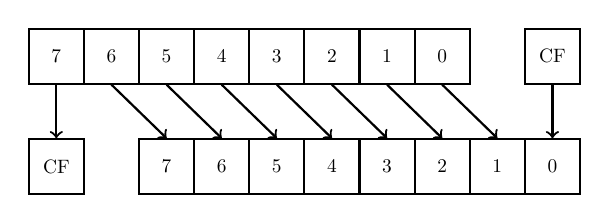
\begin{tikzpicture}[scale=0.7, every node/.style={scale=0.7}]
	\edef\bitsize{1cm}
	\tikzstyle{byte}=[draw,minimum size=\bitsize]	
	\tikzstyle{every path}=[thick]
	
	\node [draw,rectangle,minimum size=\bitsize] (a1) {7};
	\node [draw,rectangle,minimum size=\bitsize] (a2) [right of=a1] {6};
	\node [draw,rectangle,minimum size=\bitsize] (a3) [right of=a2] {5};
	\node [draw,rectangle,minimum size=\bitsize] (a4) [right of=a3] {4};
	\node [draw,rectangle,minimum size=\bitsize] (a5) [right of=a4] {3};
	\node [draw,rectangle,minimum size=\bitsize] (a6) [right of=a5] {2};
	\node [draw,rectangle,minimum size=\bitsize] (a7) [right of=a6] {1};
	\node [draw,rectangle,minimum size=\bitsize] (a8) [right of=a7] {0};
	\node (empty1) [right of=a8] {};
	\node [rectangle,draw,minimum size=\bitsize] (acf) [right of=empty1] {CF};
	
	\node (empty) [below of=a1] {};

	\node [rectangle,draw,minimum size=\bitsize] (bcf) [below of=empty] {CF};
	\node (empty2) [right of=bcf] {};
	\node [draw,rectangle,minimum size=\bitsize] (b1) [right of=empty2] {7};
	\node [draw,rectangle,minimum size=\bitsize] (b2) [right of=b1] {6};
	\node [draw,rectangle,minimum size=\bitsize] (b3) [right of=b2] {5};
	\node [draw,rectangle,minimum size=\bitsize] (b4) [right of=b3] {4};
	\node [draw,rectangle,minimum size=\bitsize] (b5) [right of=b4] {3};
	\node [draw,rectangle,minimum size=\bitsize] (b6) [right of=b5] {2};
	\node [draw,rectangle,minimum size=\bitsize] (b7) [right of=b6] {1};
	\node [draw,rectangle,minimum size=\bitsize] (b8) [right of=b7] {0};
	
	\draw [->] (a1.south) -- (bcf.north); % 7
	\draw [->] (a2.south) -- (b1.north); % 6
	\draw [->] (a3.south) -- (b2.north);
	\draw [->] (a4.south) -- (b3.north);
	\draw [->] (a5.south) -- (b4.north);
	\draw [->] (a6.south) -- (b5.north);
	\draw [->] (a7.south) -- (b6.north);
	\draw [->] (a8.south) -- (b7.north);
	\draw [->] (acf.south) -- (b8.north);

	\end{tikzpicture}
\end{center}

  \item[RCR] (M) \RU{вращать биты направо через флаг CF}\EN{rotate right via CF flag}:

\begin{center}
	\begin{tikzpicture}[scale=0.7, every node/.style={scale=0.7}]
	\edef\bitsize{1cm}
	\tikzstyle{byte}=[draw,minimum size=\bitsize]	
	\tikzstyle{every path}=[thick]

	\node [rectangle,draw,minimum size=\bitsize] (acf) {CF};
	\node (empty1) [right of=acf] {};
	
	\node [draw,rectangle,minimum size=\bitsize] (a1) [right of=empty1] {7};
	\node [draw,rectangle,minimum size=\bitsize] (a2) [right of=a1] {6};
	\node [draw,rectangle,minimum size=\bitsize] (a3) [right of=a2] {5};
	\node [draw,rectangle,minimum size=\bitsize] (a4) [right of=a3] {4};
	\node [draw,rectangle,minimum size=\bitsize] (a5) [right of=a4] {3};
	\node [draw,rectangle,minimum size=\bitsize] (a6) [right of=a5] {2};
	\node [draw,rectangle,minimum size=\bitsize] (a7) [right of=a6] {1};
	\node [draw,rectangle,minimum size=\bitsize] (a8) [right of=a7] {0};
	
	\node (empty) [below of=a1] {};

	\node [draw,rectangle,minimum size=\bitsize] (b1) [below of=empty] {7};
	\node [draw,rectangle,minimum size=\bitsize] (b2) [right of=b1] {6};
	\node [draw,rectangle,minimum size=\bitsize] (b3) [right of=b2] {5};
	\node [draw,rectangle,minimum size=\bitsize] (b4) [right of=b3] {4};
	\node [draw,rectangle,minimum size=\bitsize] (b5) [right of=b4] {3};
	\node [draw,rectangle,minimum size=\bitsize] (b6) [right of=b5] {2};
	\node [draw,rectangle,minimum size=\bitsize] (b7) [right of=b6] {1};
	\node [draw,rectangle,minimum size=\bitsize] (b8) [right of=b7] {0};
	
	\node (empty2) [right of=b7] {};
	
	\node [rectangle,draw,minimum size=\bitsize] (bcf) [right=of empty2] {CF};
	
	\draw [->] (acf.south) -- (b1.north);
	\draw [->] (a1.south) -- (b2.north);
	\draw [->] (a2.south) -- (b3.north);
	\draw [->] (a3.south) -- (b4.north);
	\draw [->] (a4.south) -- (b5.north);
	\draw [->] (a5.south) -- (b6.north);
	\draw [->] (a6.south) -- (b7.north);
	\draw [->] (a7.south) -- (b8.north);
	\draw [->] (a8.south) -- (bcf.north);

	\end{tikzpicture}
\end{center}


\myindex{x86!\Instructions!ROL}
\myindex{x86!\Instructions!ROR}
\label{ROL_ROR}
\item[ROL/ROR] (M) \RU{циклический сдвиг}\EN{cyclic shift}
  
ROL: \RU{вращать налево}\EN{rotate left}:

\input{rotate_left}

ROR: \RU{вращать направо}\EN{rotate right}:

\input{rotate_right}

\RU{Не смотря на то что многие \ac{CPU} имеют эти инструкции, в \CCpp нет соответствующих операций,
так что компиляторы с этих \ac{PL} обычно не генерируют код использующий эти инструкции}\EN{Despite the 
fact that almost all \ac{CPU}s have these instructions, there are no corresponding
operations in \CCpp, so the compilers of these \ac{PL}s usually do not generate these 
instructions}.

\RU{Чтобы программисту были доступны эти инструкции, в \ac{MSVC} есть псевдофункции}
\EN{For the programmer's convenience, at least \ac{MSVC} has the pseudofunctions} (compiler intrinsics)
\IT{\_rotl()} \AndENRU \IT{\_rotr()}\FNMSDNROTxURL{},
\RU{которые транслируются компилятором напрямую в эти инструкции}
\EN{which are translated by the compiler directly to these instructions}.


\myindex{x86!\Instructions!SAL}
  \item[SAL] \RU{Арифметический сдвиг влево}\EN{Arithmetic shift left}, \RU{синонимично}\EN{synonymous to} \TT{SHL}

\index{x86!\Instructions!SAR}
  \item[SAR] Arithmetic Shift Right

\myindex{x86!\Instructions!SETcc}
  \item[SETcc] op: \RU{загрузить 1 в op (только байт) если условие верно или 0 если наоборот}
  \EN{load 1 to operand (byte only) if the condition is true or zero otherwise}.
  \RU{Коды точно такие же, как и в инструкциях Jcc}\EN{The condition codes are the same as in the Jcc instructions} 
  (\myref{Jcc}).


\myindex{x86!\Instructions!STC}
\myindex{x86!\Flags!CF}
  \item[STC] (M) \RU{установить флаг CF}\EN{set CF flag}

\myindex{x86!\Instructions!STD}
\myindex{x86!\Flags!DF}
  \item[STD] (M) \RU{установить флаг DF}\EN{set DF flag}.
   \RU{Эта инструкция не генерируется компиляторами и вообще редкая.}
   \EN{This instruction is not generated by compilers and generally rare.}
   \RU{Например, она может быть найдена в файле}\EN{For example, it can be found in the} 
   \TT{ntoskrnl.exe} \RU{(ядро Windows) в написанных вручную функциях копирования 
   памяти}\EN{Windows kernel file, in the hand-written memory copy routines}.

\index{x86!\Instructions!STI}
  \item[STI] (M) \IFRU{установить флаг IF}{set IF flag}

\myindex{x86!\Instructions!SYSCALL}
  \item[SYSCALL] (AMD) \RU{вызов сисколла}\EN{call syscall} (\myref{syscalls})

\index{x86!\Instructions!SYSENTER}
  \item[SYSENTER] (Intel) \IFRU{вызов сисколла}{call syscall} (\ref{syscalls})

\index{x86!\Instructions!UD2}
  \item[UD2] (M) \RU{неопределенная инструкция, вызывает исключение. применяется для тестирования.}
  \EN{undefined instruction, raises exception. used for testing.}

\end{description}

\subsection{\IFRU{Инструкции FPU}{FPU instructions}}

\IFRU{-R в названии инструкции обычно означает что операнды поменяны местами, -P означает
что один элемент выталкивается из стека после исполнения инструкции, -PP означает что
выталкиваются два элемента}
{-R in mnemonic usually means that operands are reversed, -P means that one element is popped
from the stack after instruction execution, -PP means that two elements are popped}.

-P \IFRU{инструкции часто бывают полезны, когда нам уже больше не нужно хранить значение в FPU-стеке}
{instructions are often useful when we do not need a value in the FPU stack to be present anymore}.

\begin{description}
\index{x86!\Instructions!FABS}
  \item[FABS] \IFRU{заменить значение в ST(0) на абсолютное значение ST(0)}{replace value in ST(0) by absolute value in ST(0)}

\myindex{x86!\Instructions!FADD}
\myindex{x86!\Instructions!FADDP}
  \item[FADD] op: ST(0)=op+ST(0)
  \item[FADD] ST(0), ST(i): ST(0)=ST(0)+ST(i)
  \item[FADDP] ST(1)=ST(0)+ST(1);
  \RU{вытолкнуть один элемент из стека, таким образом, складываемые значения в стеке заменяются
  суммой}\EN{pop one element from the stack, i.e., the values in the stack are replaced by their sum}

 % + FADDP
\myindex{x86!\Instructions!FCHS}
  \item[FCHS] ST(0)=-ST(0)


\index{x86!\Instructions!FCOM}
\index{x86!\Instructions!FCOMP}
  \item[FCOM] \IFRU{сравнить}{compare} ST(0) \IFRU{с}{with} ST(1)
  \item[FCOM] op: \IFRU{сравнить}{compare} ST(0) \IFRU{с}{with} op
  \item[FCOMP] \IFRU{сравнить}{compare} ST(0) \IFRU{с}{with} ST(1); \IFRU{вытолкнуть один элемент из стека}
  {pop one element from the stack}
 % + FCOMP + FCOMPP
\index{x86!\Instructions!FDIVR}
  \item[FDIVR] op: ST(0)=op/ST(0)
  \item[FDIVR] ST(i), ST(j): ST(i)=ST(j)/ST(i)

 % + FDIVRP
\myindex{x86!\Instructions!FDIV}
\myindex{x86!\Instructions!FDIVP}
  \item[FDIV] op: ST(0)=ST(0)/op
  \item[FDIV] ST(i), ST(j): ST(i)=ST(i)/ST(j)
  \item[FDIVP] ST(1)=ST(0)/ST(1); \RU{вытолкнуть один элемент из стека, таким образом, 
  делимое и делитель в стеке заменяются частным}\EN{pop one element from the stack, i.e., 
  the dividend and divisor values in the stack are replaced by quotient}
 % + FDIVP
\index{x86!\Instructions!FILD}
  \item[FILD] op: \IFRU{сконвертировать целочисленный op и затолкнуть его в стек}
  {convert integer and push it to the stack}.


\myindex{x86!\Instructions!FIST}
\myindex{x86!\Instructions!FISTP}
  \item[FIST] op: \RU{конвертировать}\EN{convert} ST(0) \RU{в целочисленное}\EN{to integer} op
  \item[FISTP] op: \RU{конвертировать}\EN{convert} ST(0) \RU{в целочисленное}\EN{to integer} op; 
  \RU{вытолкнуть один элемент из стека}\EN{pop one element from the stack}
 % + FISTP
\myindex{x86!\Instructions!FLD1}
  \item[FLD1] \RU{затолкнуть 1 в стек}\EN{push 1 to stack}


\index{x86!\Instructions!FLDCW}
  \item[FLDCW] op: \IFRU{загрузить}{load} FPU control word (\ref{FPU_control_word}) \IFRU{из}{from} 16-bit op.


\myindex{x86!\Instructions!FLDZ}
  \item[FLDZ] \RU{затолкнуть ноль в стек}\EN{push zero to stack}



\index{x86!\Instructions!FLD}
  \item[FLD] op: \IFRU{затолкнуть op в стек}{push op to the stack}.

\index{x86!\Instructions!FMUL}
  \item[FMUL] op: ST(0)=ST(0)*op
  \item[FMUL] ST(i), ST(j): ST(i)=ST(i)*ST(j)
 % + FMULP
\myindex{x86!\Instructions!FSINCOS}
  \item[FSINCOS]: tmp=ST(0); ST(1)=sin(tmp); ST(0)=cos(tmp)


\myindex{x86!\Instructions!FSQRT}
  \item[FSQRT]: $ST(0)=\sqrt{ST(0)}$


\myindex{x86!\Instructions!FSTCW}
\myindex{x86!\Instructions!FNSTCW}
  \item[FSTCW] op: \RU{записать}\EN{store} FPU control word (\myref{FPU_control_word}) \RU{в}\EN{into} 16-bit op
  \RU{после проверки ожидающих исключений}\EN{after checking for pending exceptions}.
  \item[FNSTCW] op: \RU{записать}\EN{store} FPU control word (\myref{FPU_control_word}) \RU{в}\EN{into} 16-bit op.

 % + FNSTCW
\index{x86!\Instructions!FSTSW}
\index{x86!\Instructions!FNSTSW}
  \item[FSTSW] op: \IFRU{записать}{store} FPU status word (\ref{FPU_status_word}) \IFRU{в}{into} 16-bit op
  \IFRU{после проверки ожидающих исключений}{after checking for pending exceptions}.
  \item[FNSTSW] op: \IFRU{записать}{store} FPU status word (\ref{FPU_status_word}) \IFRU{в}{into} 16-bit op.

 % + FNSTSW
\myindex{x86!\Instructions!FST}
\myindex{x86!\Instructions!FSTP}
  \item[FST] op: \RU{копировать}\EN{copy} ST(0) \RU{в}\EN{to} op
  \item[FSTP] op: \RU{копировать}\EN{copy} ST(0) \RU{в}\EN{to} op; \RU{вытолкнуть один элемент из стека}
  \EN{pop one element from the stack}

\index{x86!\Instructions!FSUBR}
\index{x86!\Instructions!FSUBRP}
  \item[FSUBR] op: ST(0)=op-ST(0)
  \item[FSUBR] ST(0), ST(i): ST(0)=ST(i)-ST(0)
  \item[FSUBRP] ST(1)=ST(0)-ST(1);
  \IFRU{вытолкнуть один элемент из стека, таким образом, складываемые значения в стеке заменяются
  разностью}{pop one element from the stack, i.e., summed values in the stack are replaced by difference}

 % + FSUBRP
\index{x86!\Instructions!FSUB}
\index{x86!\Instructions!FSUBP}
  \item[FSUB] op: ST(0)=ST(0)-op
  \item[FSUB] ST(0), ST(i): ST(0)=ST(0)-ST(i)
  \item[FSUBP] ST(1)=ST(1)-ST(0);
  \IFRU{вытолкнуть один элемент из стека, таким образом, складываемые значения в стеке заменяются
  разностью}{pop one element from the stack, i.e., summed values in the stack are replaced by difference}

 % + FSUBP
\index{x86!\Instructions!FUCOM}
\index{x86!\Instructions!FUCOMP}
\index{x86!\Instructions!FUCOMPP}
  \item[FUCOM] ST(i): \IFRU{сравнить}{compare} ST(0) \AndENRU ST(i)
  \item[FUCOM]: \IFRU{сравнить}{compare} ST(0) \AndENRU ST(1)
  \item[FUCOMP]: \IFRU{сравнить}{compare} ST(0) \AndENRU ST(1); \IFRU{вытолкнуть один элемент из стека}{pop one element from stack}.
  \item[FUCOMPP]: \IFRU{сравнить}{compare} ST(0) \AndENRU ST(1); \IFRU{вытолкнуть два элемента из стека}{pop two elements from stack}.
 
  \IFRU{Инструкция работает так же как и FCOM, за тем исключением что исключение срабатывает только
  если один из операндов SNaN, но числа QNaN нормально обрабатываются}{The instructions performs just like FCOM, but exception is raised only if one of operands is SNaN,
  while QNaN numbers are processed smoothly}.
 % + FUCOMP + FUCOMPP
\index{x86!\Instructions!FXCH}
  \item[FXCH] ST(i) \IFRU{обменять местами значения в ST(0) и ST(i)}{exchange values in ST(0) and ST(i)}
  \item[FXCH] \IFRU{обменять местами значения в ST(0) и ST(1)}{exchange values in ST(0) and ST(1)}


\end{description}

\subsection{\IFRU{SIMD-инструкции}{SIMD instructions}}

% TODO

%\begin{description}
%\input{appendix/x86/instructions/DIVSD}
%\input{appendix/x86/instructions/MOVDQA}
%\input{appendix/x86/instructions/MOVDQU}
%\input{appendix/x86/instructions/PADDD}
%\input{appendix/x86/instructions/PCMPEQB}
%\input{appendix/x86/instructions/PLMULHW}
%\input{appendix/x86/instructions/PLMULLD}
%\input{appendix/x86/instructions/PMOVMSKB}
%\input{appendix/x86/instructions/PXOR}
%\end{description}

% SHLD !
% SHRD !
% BSWAP !
% CMPXCHG
% XADD !
% CMPXCHG8B
% RDTSC !
% PAUSE!

% xsave
% fnclex, fnsave
% movsxd, movaps, wait, sfence, lfence, pushfq
% prefetchw
% REP RETN
% REP BSF
% movnti, movntdq, rdmsr, wrmsr
% ldmxcsr, stmxcsr, invlpg
% swapgs
% movq, movd
% mulsd
% POR
% IRETQ
% pslldq
% psrldq
% cqo, fxrstor, comisd, xrstor, wbinvd, movntq
% fprem
% addsb, subsd, frndint

% rare:
%\item[ENTER]
%\item[LES]
% LDS
% XLAT

\subsection{\IFRU{Инструкции с печатаемым ASCII-опкодом}{Instructions having printable ASCII opcode}}

(\IFRU{В 32-битном режиме}{In 32-bit mode}).

\label{printable_x86_opcodes}
\index{Shellcode}
\IFRU{Это может пригодиться для создания шеллкодов}{It can be suitable for shellcode constructing}.
\IFRU{См. также}{See also}: \ref{subsec:EICAR}.

% FIXME: break table
\begin{center}
\begin{longtable}{ | l | l | l | }
\hline
\cellcolor{blue!25} ASCII\IFRU{-символ}{ character} & 
\cellcolor{blue!25} \IFRU{шестнадцатеричный код}{hexadecimal code} & 
\cellcolor{blue!25} x86\IFRU{-инструкция}{ instruction} \\
\hline
0	 &30	 &XOR \\
1	 &31	 &XOR \\
2	 &32	 &XOR \\
3	 &33	 &XOR \\
4	 &34	 &XOR \\
5	 &35	 &XOR \\
7	 &37	 &AAA \\
8	 &38	 &CMP \\
9	 &39	 &CMP \\
:	 &3a	 &CMP \\
;	 &3b	 &CMP \\
<	 &3c	 &CMP \\
=	 &3d	 &CMP \\
?	 &3f	 &AAS \\
@	 &40	 &INC \\
A	 &41	 &INC \\
B	 &42	 &INC \\
C	 &43	 &INC \\
D	 &44	 &INC \\
E	 &45	 &INC \\
F	 &46	 &INC \\
G	 &47	 &INC \\
H	 &48	 &DEC \\
I	 &49	 &DEC \\
J	 &4a	 &DEC \\
K	 &4b	 &DEC \\
L	 &4c	 &DEC \\
M	 &4d	 &DEC \\
N	 &4e	 &DEC \\
O	 &4f	 &DEC \\
P	 &50	 &PUSH \\
Q	 &51	 &PUSH \\
R	 &52	 &PUSH \\
S	 &53	 &PUSH \\
T	 &54	 &PUSH \\
U	 &55	 &PUSH \\
V	 &56	 &PUSH \\
W	 &57	 &PUSH \\
X	 &58	 &POP \\
Y	 &59	 &POP \\
Z	 &5a	 &POP \\
\lbrack{}	 &5b	 &POP \\
\textbackslash{}	 &5c	 &POP \\
\rbrack{}	 &5d	 &POP \\
\verb|^|	 &5e	 &POP \\
\_	 &5f	 &POP \\
\verb|`|	 &60	 &PUSHA \\
a	 &61	 &POPA \\
f	 &66	 &\IFRU{(в 32-битном режиме) переключиться на}{(in 32-bit mode) switch to}\\
   & & \IFRU{16-битный размер операнда}{16-bit operand size} \\
g	 &67	 &\IFRU{(в 32-битном режиме) переключиться на}{in 32-bit mode) switch to}\\
   & & \IFRU{16-битный размер адреса}{16-bit address size} \\
h	 &68	 &PUSH\\
i	 &69	 &IMUL\\
j	 &6a	 &PUSH\\
k	 &6b	 &IMUL\\
p	 &70	 &JO\\
q	 &71	 &JNO\\
r	 &72	 &JB\\
s	 &73	 &JAE\\
t	 &74	 &JE\\
u	 &75	 &JNE\\
v	 &76	 &JBE\\
w	 &77	 &JA\\
x	 &78	 &JS\\
y	 &79	 &JNS\\
z	 &7a	 &JP\\
\hline
\end{longtable}
\end{center}

\index{x86!\Instructions!AAA}
\index{x86!\Instructions!AAS}
\index{x86!\Instructions!CMP}
\index{x86!\Instructions!DEC}
\index{x86!\Instructions!IMUL}
\index{x86!\Instructions!INC}
\index{x86!\Instructions!JA}
\index{x86!\Instructions!JAE}
\index{x86!\Instructions!JB}
\index{x86!\Instructions!JBE}
\index{x86!\Instructions!JE}
\index{x86!\Instructions!JNE}
\index{x86!\Instructions!JNO}
\index{x86!\Instructions!JNS}
\index{x86!\Instructions!JO}
\index{x86!\Instructions!JP}
\index{x86!\Instructions!JS}
\index{x86!\Instructions!POP}
\index{x86!\Instructions!POPA}
\index{x86!\Instructions!PUSH}
\index{x86!\Instructions!PUSHA}
\index{x86!\Instructions!XOR}

\IFRU{В итоге}{Summarizing}:
AAA, AAS, CMP, DEC, IMUL, INC, JA, JAE, JB, JBE, JE, JNE, JNO, JNS, JO, JP, JS, POP, POPA, PUSH, PUSHA, 
XOR.

